\documentclass[a4paper, 10pt, notitlepage]{article}

\usepackage{moreverb} %para importar codigo

\usepackage{pepotina} %paquete personal para la caratula del DC

\usepackage[spanish,activeacute]{babel}
\usepackage{babel} %paquete de idioma

\usepackage[latin1]{inputenc}

%\usepackage{color}

\usepackage{hyperref}
%\usepackage[all]{hypcap}

\usepackage{caeycaeING}

\usepackage{fancyhdr} %linea sup con comentarios

\usepackage{lscape} %para hoja apaisada

\usepackage{framed} %para crear cajas de texto

\usepackage{lastpage} %ultima pagina

%\usepackage{pstricks}
%\usepackage{uml} %UML

\usepackage{listings}
%\lstset{
%  breaklines=true,                                     % line wrapping on
%  language=ocl,
%  frame=ltrb,
%  framesep=5pt,
%  basicstyle=\normalsize,
%  keywordstyle=\ttfamily\color{OliveGreen},
%  identifierstyle=\ttfamily\color{CadetBlue}\bfseries,
%  commentstyle=\color{Brown},
%  stringstyle=\ttfamily,
%  showstringspaces=ture
%}

\addtolength{\topmargin}{-50pt} 
\addtolength{\textwidth}{105pt}
\addtolength{\textheight}{120pt}
\addtolength{\oddsidemargin}{-50pt}

%\newcommand{\minix}{\textsl{minix }}

%%% Encabezado y pie de p'agina
\pagestyle{fancy}
\fancyhead[LO]{Ingenieria del Software I}
\fancyhead[C]{}
\fancyhead[RO]{P\'agina \thepage\ de \pageref{LastPage}}
\renewcommand{\headrulewidth}{0.4pt}
\fancyfoot{}

\newcommand{\depto}{{\bf DPTO: }}


\def\falta#1{ \begin{framed}	\begin{center} \hspace{1cm} \Large FALTA \normalsize #1 \hspace{1cm} \end{center} \end{framed}}


\def\imagen#1#2#3{\vskip0.5cm
{\large #3}
\begin{center}
\includegraphics[scale=#1]{#2}
\end{center}}


\begin{document}

\universidad{Universidad de Buenos Aires}
\facultad{Facultad de ciencias exactas y naturales}
\departamento{Departamento de Computacion}
\materia{Ingenieria del Software I}
\resumen{Proyecto casino online}
\keys{UML, Objetivos, Agentes, Casos De Uso, Diagrama De Contexto, Modelo Conceptual, OCL, Diagrama de Actividades, FSM}
\titulo{Proyecto: Casino Online}
\subtitulo{Informe 1: Analisis de Requerimientos y especificaci�n}
\grupo{Numero de grupo: 2}
\fecha{1er Cuatrimeste 2008}
\footspace{1cm}
\integrante{Aquino, Isis}{313/05}{isisaquino@yahoo.com.ar}
\integrante{Alvarez, Maria de los Angeles}{264/05}{mdelosaalvarez@hotmail.com}
\integrante{Engler, Christian Alejandro}{314/05}{caeycae@gmail.com}

%caratula
\maketitle{}

\tableofcontents


\section{Introducci�n}




\section{Dise�o por funcionalidad}

\subsection{Registracion y Ingreso al casino online y modificacion de saldo}

\subsubsection{Registracion}

Segun lo acordado en la especificacion, la registracion de los usuarios se hace por fuera del sistema informatico del casino online.\\
En el momento de abrir el casino el sistema contar� con un archivo XML (en el futuro podria ser de otra manera)
\\
\textbf{Dicho archivo tendr� la siguiente sintaxis:}

\begin{verbatim}
<jugadores>
    <jugador nombre="Nombre" saldo"valor numerico del saldo" vip="true | false">
</jugadores>
\end{verbatim}

\subsubsection{Modificacion de saldo}

Las modificaciones de saldo real solo se pueden realizar mientras el casino permanece cerrado.\\
Mas alla de la operatoria, debar� modificarse el archivo definido en el punto anterior con el monto correspondiente antes de la proxima apertura del casino.

\subsubsection{Ingreso y egreso del casino}

En esta seccion estamos apuntando al ingreso de jugadores al casino (no al ingreso de jugadores observadores, dicha interaccion con el casino esta mostrada en la seccion Invitado)

Presentamos aqui diagramas de secuencia del correcto ingreso al casino online.

\newpage
\imagen{0.5}{img/entrar.png}{Jugador entrando al casino aceptado}
\falta{entrar erroneo}

\newpage
\imagen{0.5}{img/salir.png}{Jugador saliendo al casino aceptado}
\falta{salir erroneo}


\newpage
\subsection{Administracion del Casino}

\subsubsection{Apertura del casino}

\begin{verbatim}
<valorFichas>
        <valorFicha valor="" />
</valorFichas>
<probablilidades>
    <jugadaFeliz proba="" montoMinimo="" />
    <jugadaTodosPonen proba="" />
    <jugadaNormal proba=""  />
    <craps>
        <valorDado numero="1" proba="" />
        .
        .
        <valorDado numero="6" proba="" />
    </craps>
    <traga>
        <gordoProgresivo montoMinimo="" descuento=""/>
        <combinaciones>
            <combinacion simbolo1="" simbolo2="" simbolo3="" proba=""/>
        </combinaciones>
    </traga>
</probablilidades>
\end{verbatim}

\falta{TODO lo de apertura del casino}

\subsubsection{Clausura del casino}

\falta{TODO lo de apertura del casino}

\subsection{Invitado}









%%\section{Escenarios en castellano y Diagramas de secuencias de operaciones mas relevantes}
%%
%%\section{Pseudocodigo de operaciones mas complicadas en lo algoritmico}
%%
%%\section{Justificacion, analisis y explicacion de su dise�o}
%%
%%\section{Trazabilidad completa con informe 1}
%%
%%\section{Conclusiones}

%%%- Introduccion. Cambios con respecto al informe 1.
%%%- .
%%%- Pseudocodigo de operaciones mas complicadas en lo algoritmico.
%%%- Diagrama de clases junto una explicacion en castellano de que hace y para sirve cada clase, y de los aspectos mas interesantes del diagrama. Es buena idea factorizar/separar el/los diagramas en base a algun criterio para mostrarlos con mas claridad. Si su dise�o tiene mas de un paquete seria interesante ver las dependencias entre paquetes...
%%%- Justificacion, analisis y explicacion de su dise�o, utilizando desde principios de dise�o, hasta patterns, pasando por depedencias, acoplamiento y cohesion, hasta mas secuencias de ejemplo para explicar porque su dise�o es bueno y elegante al resolver los problemas que se les presentaron.
%%%- Trazabilidad completa con informe 1. Ademas todo el informe va dirigido al area de sistemas de la empresa de los socios.
%%%- Conclusiones.
%%%
%%%Saludos,
%%%Nicolas.






%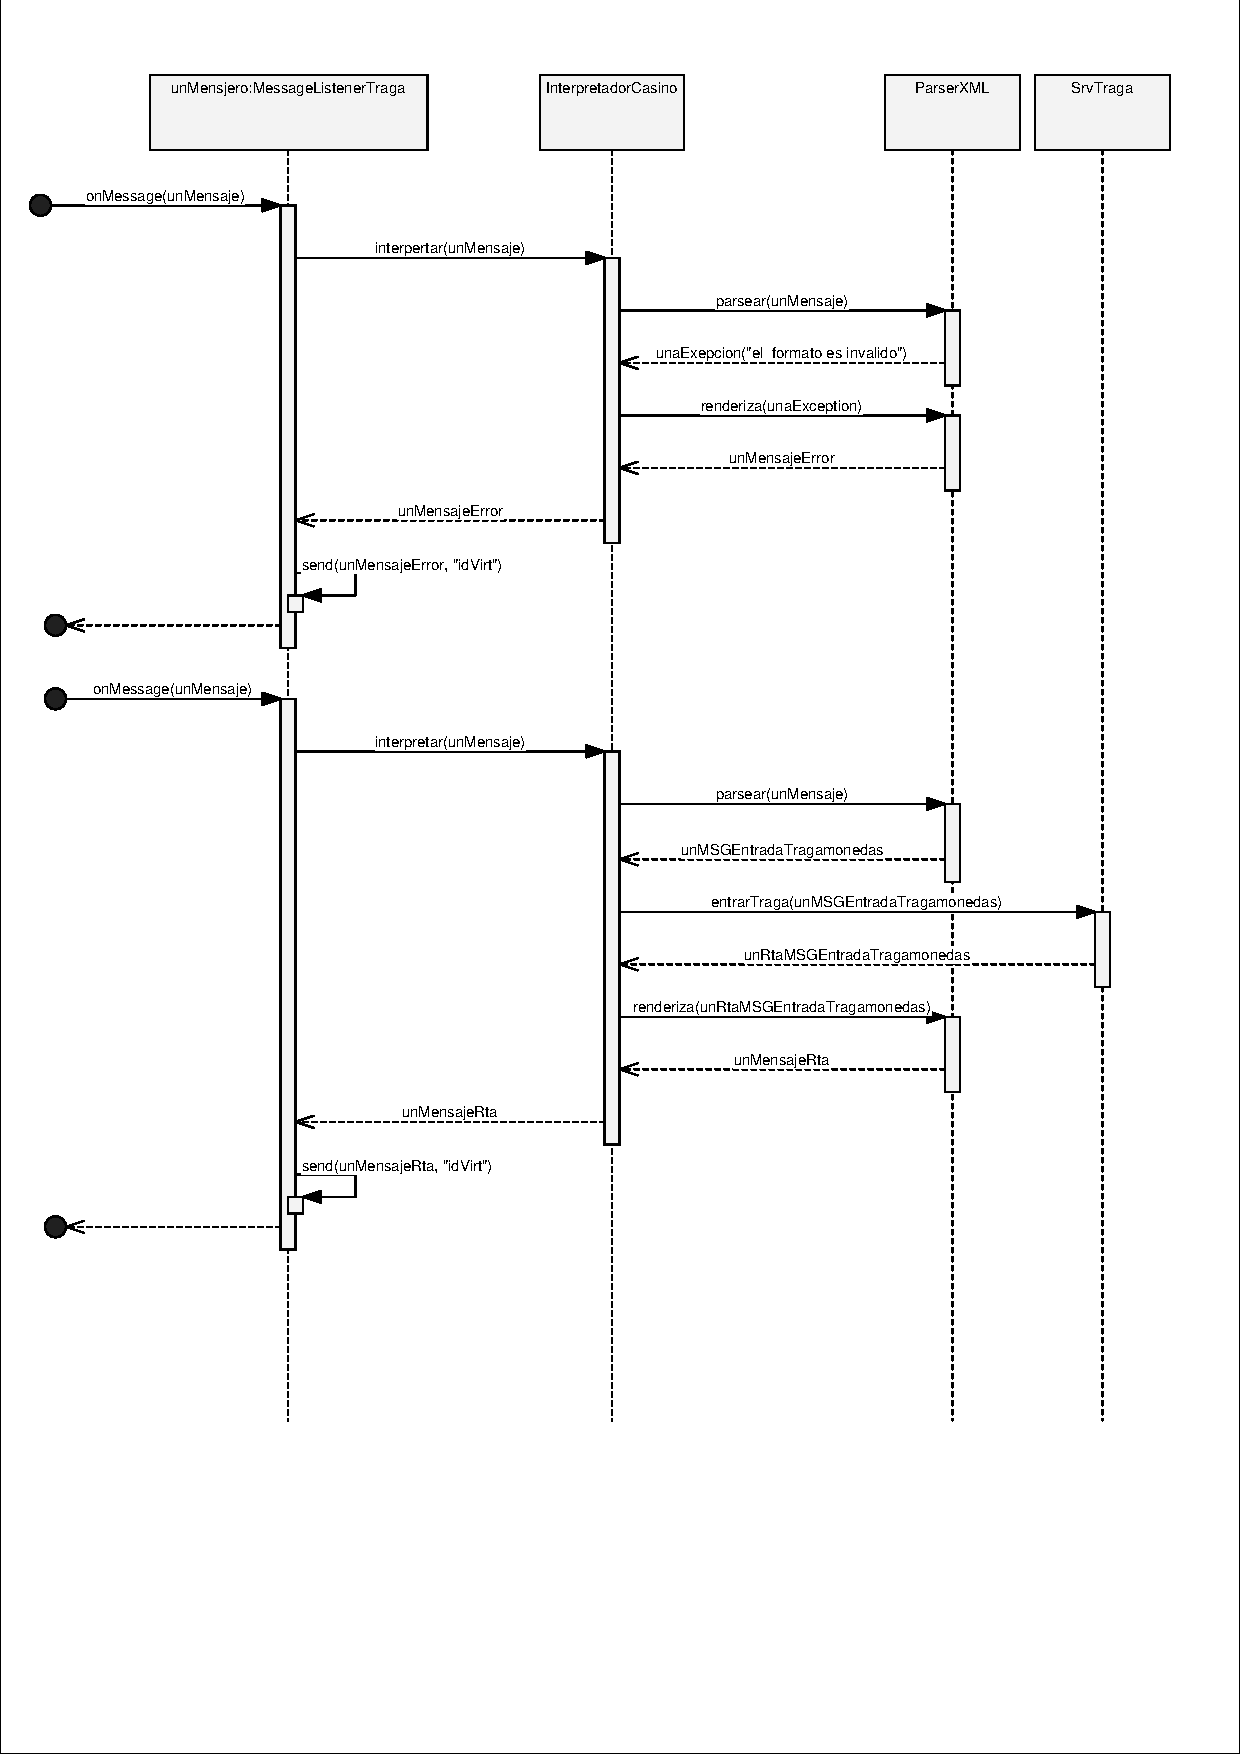
\includegraphics[scale=0.60]{mensajero.pdf}
%,angle=90]
%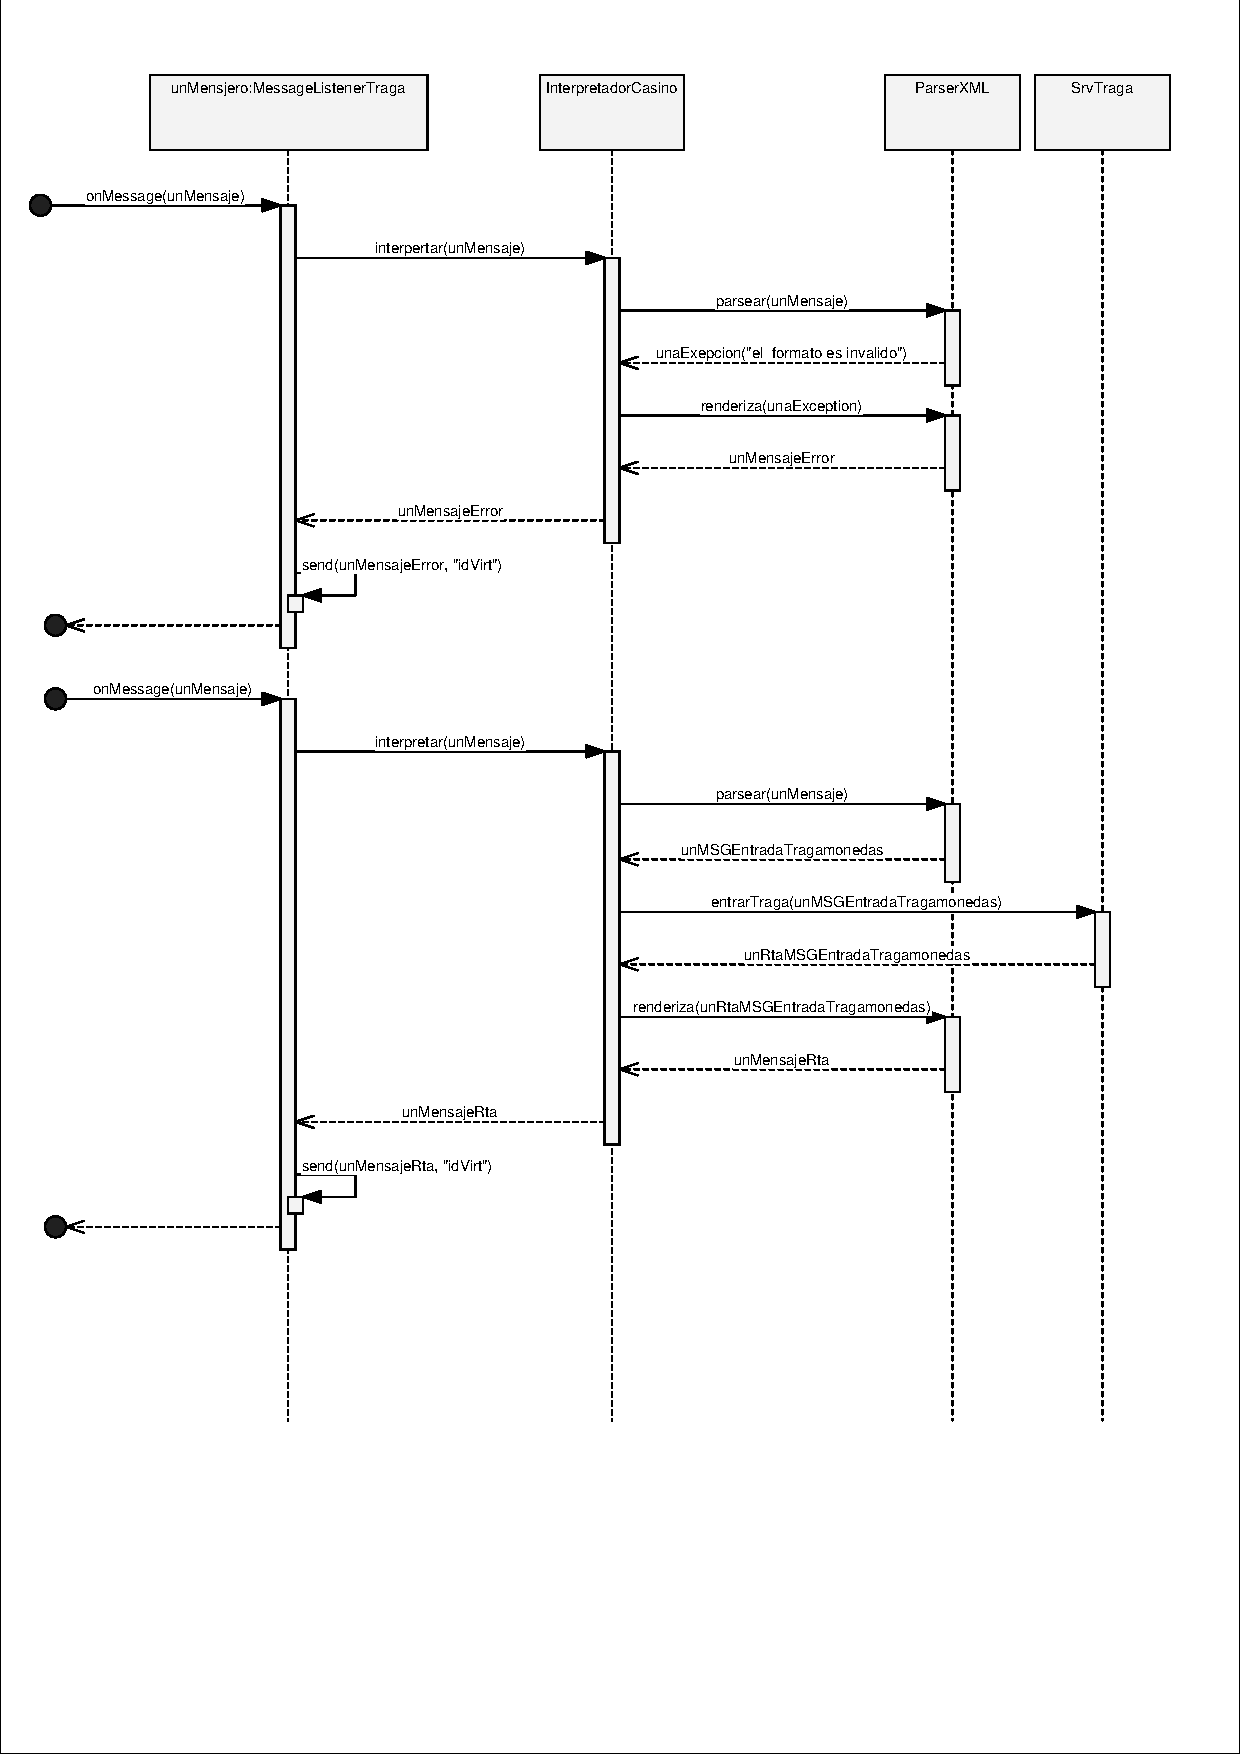
\includegraphics[height=4in,width=6in]{mensajero.pdf}
%  \includegraphics[height=60mm]{myfig.eps}
%  \includegraphics[scale=0.75]{myfig.eps}
%  \includegraphics[angle=45,width=52mm]{myfig.eps}


\end{document}


